\documentclass{article}
\usepackage{hyperref}
\usepackage{amsmath}
\usepackage{amssymb}
\usepackage{pgfplots}
\usepackage{float}
\usepackage{todonotes}
\usepackage{tikz}
\usepackage[shortlabels]{enumitem}

% For InkScape tex files:
\usepackage[pdf]{pstricks}

\renewcommand{\Re}{\mathbb{R}}
\newcommand{\Li}{\mathcal{L}}
\newcommand{\Ex}{\mathbb{E}}
\renewcommand{\Pr}{\mathbb{P}}
\newcommand{\Hy}{\mathcal{H}}
\newcommand{\sign}{\text{sign}}
\newcommand{\error}{\text{error}}

\newcommand\bigO[1]{
    \ensuremath{\mathcal{O}\left(#1\right)}
    }

\newcommand{\sigmoidPlot}{
    
    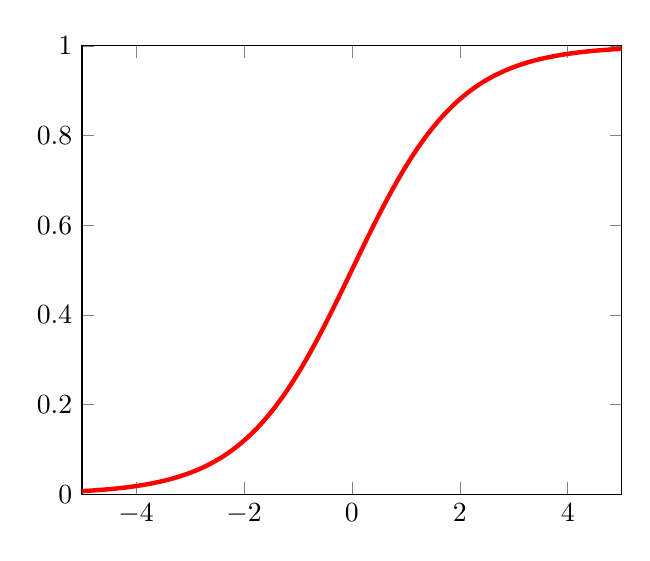
\begin{tikzpicture}
        \begin{axis}[xmin=-5, xmax=5, ymin=0, ymax=1, samples=150]
        \addplot[red, ultra thick] {1/(1+exp(-x))};
        \end{axis}
    \end{tikzpicture}
    
    }

\usetikzlibrary{positioning, calc}
\usetikzlibrary{arrows.meta}

\tikzstyle{circlebox}=[circle,thick,draw=black!75,minimum size=8mm]
\tikzstyle{inputnode}=[circlebox, draw=blue!75]
\tikzstyle{hiddennode}=[circlebox, draw=orange!75]
\tikzstyle{outputnode}=[circlebox, draw=orange!75]
\tikzstyle{simplebox}=[rectangle,thick,draw=black!75,
fill=black!20,minimum size=4mm]
\tikzstyle{textbox}=[rectangle,thick,minimum size=4mm,draw=black!0,
fill=black!0]
\tikzstyle{halfvdistance}=[yshift=-0.7cm]
\tikzstyle{abovebetween}=[xshift=-2.7mm]
\tikzstyle{edgepath} = [-Latex,->,shorten >=1pt,-stealth,semithick, rounded 
corners=5pt]

\def \nodedv {0.735cm}
\def \nodedh {0.65cm}

\tikzset{
    between/.style args={#1 and #2}{
        at = ($(#1)!0.5!(#2)$)
    }
}